\documentclass[10pt,journal]{IEEEtran}
\usepackage{amsmath,amssymb,amsthm}
\usepackage{graphicx}
\usepackage{booktabs}
\usepackage{array}
\usepackage{url}
\usepackage{cite}
\usepackage{placeins}
\graphicspath{{./}{./fig/}}
\renewcommand{\arraystretch}{1.1}
\newtheorem{proposition}{Proposition}
\newcommand{\mmax}{m_{\max}}
\hyphenation{Insertion Mahonian}

\begin{document}

\title{Entropy Landscapes and Kinetics of Classical Sorting Algorithms}
\author{Punyajit Mishra% TODO before submission: add affiliation, city/country, e-mail (and ORCID if available)
\thanks{Manuscript dated September 28, 2026.}}
\markboth{Entropy Landscapes and Kinetics of Classical Sorting Algorithms}{Mishra}
\maketitle

\begin{abstract}
Sorting algorithms are usually compared by asymptotic complexity, which says little about how a particular run moves through the space of array arrangements. We treat a permutation of $n$ distinct keys as a microstate and its inversion count $m$ as a macrostate, with exact multiplicities $\Omega_n(m)$ from the Mahonian distribution, entropy $S(m)=\ln\Omega_n(m)$, and a normalised disorder energy $E=m/\mmax$. Instrumented Bubble, Insertion, Merge, Heap and Quick Sort record trajectories $(E_t,S_t)$ together with comparisons and writes; a cost $W=C+M$ defines the disorder removed per unit cost, $R=(E_0-E_f)/W$. We prove exactly how each algorithm's steps change $m$: Bubble and Quick Sort never increase it, Insertion and Merge Sort remove it in data-determined batches, and every sift-down swap in Heap Sort increases it. In the $n=100$ trajectory experiment over 30 uniform-random inputs, Heap Sort raises $E$ in 83.0\% of recorded steps, from $0.50$ to a mean peak of $0.79$, and traverses $3.28$ times its net entropy change, against $1.002$ for the other four. Reading an effective inverse temperature $\beta_{\mathrm{eff}}=dS/dE$ off the exact landscape shows this excursion is not merely larger but qualitatively different: the four monotone algorithms have mean most-negative $\beta_{\mathrm{eff}}\approx-3.9$, while Heap Sort's mean most-negative value is $\beta_{\mathrm{eff}}\approx-343$, nearly two orders of magnitude larger in magnitude. Cost rankings depend on input shape and size: last-pivot Quick Sort is cheapest on uniform-random input but third on nearly-sorted and on reverse-sorted input, and Insertion Sort overtakes Merge Sort in cost at $n\approx 23$. Since $R=E_0/W$ for complete sorts, $R$ normalises across input distributions but adds no ranking information beyond $W$; the entropy-path and inverse-temperature statistics do. The framework is abstract and measures no physical energy.
\end{abstract}

\begin{IEEEkeywords}
sorting algorithms, inversion count, permutation entropy, presortedness, computational kinetics, algorithmic thermodynamics
\end{IEEEkeywords}

\section{Introduction}
\IEEEPARstart{A}{lgorithms} are usually compared by how their resource use scales with input size~\cite{ref1}. Two runs with the same cost can nevertheless pass through very different sequences of intermediate arrangements, and the same algorithm can behave very differently on inputs of different shape. Adaptive sorting studies the shape dependence through measures of presortedness such as the number of inversions and the number of runs~\cite{ref33,ref34}; entropy has been used to analyse comparison sorting~\cite{ref4,ref6,ref7} and to design entropy-sensitive algorithms~\cite{ref5}. This paper adds a statistical-mechanical description of the \emph{path} an algorithm takes: how its disorder and the entropy of its current macrostate evolve while it runs.

The vocabulary is borrowed from the thermodynamics of computation, in which logically irreversible operations carry a minimum dissipation cost~\cite{ref9}, computation can in principle be made reversible~\cite{ref10}, program properties can be treated as observables of a Gibbs ensemble~\cite{ref11}, and statistical-physics methods explain phase transitions in computational hardness~\cite{ref12}. We make no physical-energy claim. A separate empirical literature measures the energy that sorting code actually draws from real hardware, for instance in energy-constrained comparison models~\cite{ref21} and on smartphones~\cite{ref22}; our framework is complementary because it instruments the abstract state space rather than a device.

\textbf{Contributions.} (i)~We compute the entropy landscape exactly with big-integer arithmetic and quantify the error of the Gaussian approximation. (ii)~We prove how each algorithm's recorded steps change the inversion count (Section~\ref{sec:struct}). (iii)~We introduce trajectory statistics, including an entropy path length that separates Heap Sort from the four algorithms whose trajectories are monotone. (iv)~We report paired experiments with 1000 trials per input distribution at $n=100$, a size sweep to $n=2000$, and pivot and run-adaptive variants. (v)~We show that the disorder reduction rate $R$ equals $E_0/W$ and therefore ranks algorithms exactly as $W$ does within a fixed distribution.

\section{Background}
\subsection{Permutations and inversions}
An inversion of a permutation $\pi$ of $n$ distinct keys is a pair of positions $i<j$ with $\pi_i>\pi_j$, and
\begin{equation}
m(\pi)=\bigl|\{(i,j):i<j,\ \pi_i>\pi_j\}\bigr|,
\label{eq:m}
\end{equation}
so $m\in\{0,\dots,\mmax\}$ with $\mmax=\binom n2$.
The sorted permutation has $m=0$ and the reverse-sorted one has $m=\mmax$. The statistic is a classical object of sorting analysis~\cite{ref1} and of enumerative combinatorics~\cite{ref14}, and the combinatorics of permutations more broadly is surveyed in~\cite{ref15}.

\subsection{Multiplicity and exact entropy}
Let $\Omega_n(m)$ be the number of permutations with $m$ inversions. These Mahonian numbers~\cite{ref13} satisfy
\begin{equation}
\sum_{m=0}^{\mmax}\Omega_n(m)\,q^m=\prod_{k=1}^{n}\frac{1-q^k}{1-q},
\label{eq:mahon}
\end{equation}
and the counts of permutations by inversions have been studied in their own right~\cite{ref16}. Ordering and mixing in a physical system of diffusing particles is analysed in~\cite{ref17}. We define the macrostate entropy in reduced units as
\begin{equation}
S(m)=\ln\Omega_n(m),\qquad \Omega_n(0)=\Omega_n(\mmax)=1 .
\label{eq:S}
\end{equation}
$\Omega_n(m)$ is symmetric about $\mmax/2$ and, for large $n$, approximately Gaussian with mean $\mu=n(n-1)/4$ and variance $\sigma^2=n(n-1)(2n+5)/72$. We do not use the Gaussian form: multiplying out~\eqref{eq:mahon} with arbitrary-precision integers is inexpensive (the $n=100$ table is built in under 0.1\,s), and Section~\ref{sec:res-entropy} shows that the Gaussian approximation is badly wrong in the tails that nearly-sorted inputs occupy. Our implementation is validated against brute-force enumeration for $n=5,6,7$ and by $\sum_m\Omega_n(m)=n!$ and symmetry at $n=100$.

\subsection{Combinatorial and Shannon entropy}
$S(m)$ is a Boltzmann-type entropy: it counts the configurations compatible with a macrostate. It is distinct from the Shannon entropy of a random variable, for which Cover and Thomas give the standard development, including mutual information and the asymptotic equipartition property~\cite{ref2}. Gray's text treats the same material with more emphasis on the entropy rates of random processes~\cite{ref3}. The two are related by a change of base, $S(m)/\ln 2$ being the number of bits needed to single out one of the $\Omega_n(m)$ permutations in the macrostate.

\subsection{Disorder energy and ensemble}
\label{sec:ensemble}
The dimensionless disorder energy is $E(\pi)=m(\pi)/\mmax\in[0,1]$. For an inverse-temperature parameter $\beta$ it defines a canonical ensemble $p_\beta(\pi)\propto e^{-\beta E(\pi)}$ with partition function $Z(\beta)=\sum_m\Omega_n(m)e^{-\beta m/\mmax}$ and free energy $F=-\beta^{-1}\ln Z$. $E$ is a chosen observable in the same sense as the observables of algorithmic thermodynamics~\cite{ref11}. The ensemble is defined for completeness; the results below use only $E$ and $S$ along trajectories.

\subsection{Thermodynamics of computation}
Landauer's bound~\cite{ref9} and Bennett's reversible computation~\cite{ref10} anchor the field. The minimal work cost of information processing has been formulated for general tasks in an information-theoretic setting~\cite{ref18}; historical accounts trace how these ideas developed at IBM~\cite{ref20}; overviews mark sixty years of Landauer's principle~\cite{ref25}, and recent work extends the thermodynamics of computation to irreversible transitions and stochastic computation times~\cite{ref28}, and~\cite{ref31} discusses the principle together with the thermodynamics of computation. A physical lower bound for a sorting run would require knowing which bits a specific machine erases; our simulation does not, so these results are background only.

\subsection{Entropy in sorting theory}
The decision-tree argument shows that any comparison sort needs at least $\log_2 n!$ comparisons in the worst case~\cite{ref1,ref8}. Kahn and Kim relate the number of comparisons needed when partial order information is available to the entropy of the incomparability graph~\cite{ref4}. Schellekens proves an entropy conservation law for comparison-based algorithms~\cite{ref6}, List \emph{et al.}\ tie the expected comparisons of randomised Quick Sort to the entropy of the pivot source~\cite{ref7}, and Gila \emph{et al.}\ define a run-based entropy for entropy-sensitive in-place sorting~\cite{ref5}. None of these tracks a scalar macrostate along a specific run, which is what we do.

\section{Framework}
\label{sec:frame}
\subsection{States and recording}
A state is recorded only when the full working array is a permutation of the input. Bubble, Quick and Heap Sort record after every swap. Insertion Sort records after each completed insertion, and Merge Sort after each completed merge; buffers containing duplicated keys are never recorded. Comparisons and writes are counted at their true frequency: a swap costs three writes, each shift or copy one write.

\subsection{Cost and disorder reduction rate}
The abstract cost is $W=C+M$, comparisons plus writes. Counting writes separately from comparisons follows the asymmetric read/write cost view of sorting~\cite{ref19}; here the two weights are equal. The disorder reduction rate is
\begin{equation}
R=\frac{E_0-E_f}{W}.
\label{eq:R}
\end{equation}
\begin{proposition}
\label{prop:R}
For an algorithm that sorts completely ($E_f=0$), $R=E_0/W$. Hence, on any fixed input, ordering algorithms by decreasing $R$ is ordering them by increasing $W$. The statement is a within-input ranking result; $R$ does not make costs from different input distributions directly comparable without specifying the starting disorder.
\end{proposition}
This is immediate from~\eqref{eq:R}. It means $R$ is a normalisation that makes costs comparable across distributions with different starting disorder; it is not an independent efficiency measure, and we never treat it as one.

\subsection{Trajectory statistics}
For a recorded sequence $m_0,m_1,\dots,m_T$ we report the number of steps $T$, the fraction of steps with $m_{t+1}>m_t$, the peak $\max_t E_t$, the largest single-step drop as a fraction of $m_0$, and the entropy path length
\begin{equation}
\Lambda=\frac{\sum_{t=0}^{T-1}\bigl|S(m_{t+1})-S(m_t)\bigr|}{S(m_0)}.
\label{eq:Lambda}
\end{equation}
For $S(m_0)>0$, every complete sort has the same net change $S(m_0)\to 0$, so $\Lambda$ measures the total entropy variation relative to the initial entropy. $\Lambda=1$ when $S$ decreases monotonically, while $\Lambda>1$ records an entropy detour, which can arise either from reversals in $S$ or from crossing the entropy peak even when $m$ itself changes monotonically. The peak and the fraction of increasing steps both characterize upward excursions in the $E$ coordinate, but they are not equivalent statistics.

We also read an effective inverse temperature off the exact landscape,
\begin{equation}
\beta_{\mathrm{eff}}(m)=\frac{dS}{dE}\bigg|_m \approx \mmax\,\frac{S(m+1)-S(m-1)}{2},
\label{eq:betaeff}
\end{equation}
a central difference defined for $0<m<\mmax$. The endpoint states $m=0$ and $m=\mmax$ therefore have no $\beta_{\mathrm{eff}}$ value under this definition and are excluded from $\beta_{\mathrm{eff}}$-based trajectory statistics. In the canonical ensemble of Section~\ref{sec:ensemble}, $\beta_{\mathrm{eff}}(m)$ is the local inverse-temperature value associated with macrostate $m$: in the continuous approximation, the modal condition is $\beta_{\mathrm{eff}}=\beta$. Thus it converts a raw inversion count into the inverse-temperature scale of the ensemble in which that count is typical. $\beta_{\mathrm{eff}}>0$ below the entropy peak and $\beta_{\mathrm{eff}}<0$ above it; for odd $\mmax$, the two central macrostates straddle $\beta_{\mathrm{eff}}=0$. Because the disorder energy is bounded, negative $\beta_{\mathrm{eff}}$ values are mathematically allowed and correspond to the high-disorder side of the landscape, not to a physically colder state. We use it to measure how far a trajectory strays from the high-entropy centre of the landscape (Section~\ref{sec:res-temp}).

\section{Structural properties of the trajectories}
\label{sec:struct}
\begin{proposition}[Swap lemma]
\label{prop:swap}
Exchanging positions $i<j$ with $\pi_i>\pi_j$ (an inverted pair) reduces the inversion count by exactly $1+2c$, where $c$ is the number of positions $k$ with $i<k<j$ and $\pi_j<\pi_k<\pi_i$. Exchanging a non-inverted pair $i<j$, $\pi_i<\pi_j$, increases it by exactly $1+2c'$ with $c'=|\{k:i<k<j,\ \pi_i<\pi_k<\pi_j\}|$.
\end{proposition}
\begin{proof}
Only pairs involving $i$ or $j$ can change. The pair $(i,j)$ itself flips. For an intermediate $k$ with value below both or above both of $\pi_i,\pi_j$, the two pairs $(i,k)$ and $(k,j)$ contribute the same number of inversions before and after. If $\pi_k$ lies strictly between the two values, the two pairs contribute two inversions when $\pi_i>\pi_j$ and none after the swap, and the reverse for the non-inverted case. Pairs with an endpoint outside $[i,j]$ are unchanged. The second statement is the first read backwards.
\end{proof}

\begin{proposition}[Bubble Sort]
Every swap lowers $m$ by exactly one, so the recorded trajectory descends linearly in exactly $m_0$ steps for every input.
\end{proposition}
\emph{Proof.} Adjacent positions have no intermediate $k$, so Proposition~\ref{prop:swap} gives $c=0$ and Bubble Sort only swaps inverted pairs. \hfill$\square$

\begin{proposition}[Quick Sort with Lomuto partition]
Every recorded nontrivial swap exchanges an inverted pair, so $m$ never increases and each nonzero drop is odd.
\end{proposition}
\emph{Proof.} Within a partition the region $\pi_i,\dots,\pi_{j-1}$ holds keys larger than the pivot. Every recorded nontrivial swap of $\pi_i$ with $\pi_j\le$ pivot therefore exchanges an inverted pair ($i<j$, $\pi_i>\pi_j$), and the nontrivial final swap of $\pi_i$ with the pivot does likewise. Self-swaps are not recorded as swaps. Apply Proposition~\ref{prop:swap}. \hfill$\square$

Individual swaps can nevertheless be long: the drop grows with the swap distance through $c$, unlike Bubble Sort's unit steps.

\begin{proposition}[Insertion Sort]
The recorded drop at the insertion of $\pi_i$ equals the number of larger keys in the sorted prefix, and the drops sum to $m_0$. There are $n-1$ recorded steps, and a step is zero when the key is already in place.
\end{proposition}
\emph{Proof.} Inserting a key into a sorted prefix removes exactly the inversions it forms with that prefix and no others. \hfill$\square$

\begin{proposition}[Merge Sort]
When the merge with split point $s$ completes, it removes exactly the cross inversions between the two halves, and every inversion $(i,j)$ is removed at the unique merge whose split separates $i$ and $j$. There are $n-1$ recorded steps, and on a uniformly random input the last merge removes on average a fraction $\tfrac{(n/2)^2/2}{n(n-1)/4}\approx\tfrac12$ of the initial inversions.
\end{proposition}
\emph{Proof.} By induction both halves are sorted when they are merged, so all their internal inversions are already zero; the merge sorts the union and leaves inversions with positions outside the block untouched. Each pair of positions is separated by exactly one recursion node, and the expected number of cross inversions between two random halves of size $n/2$ is $(n/2)^2/2$. \hfill$\square$

\begin{proposition}[Heap Sort]
Every swap inside a sift-down exchanges a parent with a strictly larger child, that is, a non-inverted pair, and therefore \emph{increases} $m$ by $1+2c'$. Only the $n-1$ root--last extraction swaps exchange an inverted pair and decrease $m$. If a run makes $s$ recorded swaps, the fraction of steps at which $m$ increases is exactly $1-(n-1)/s$.
\end{proposition}
\emph{Proof.} A max-heap sift-down moves the smaller parent below the larger child, which has a larger index. The root is the maximum of the active heap, so the extraction swap exchanges it with a smaller key at a larger index. Apply Proposition~\ref{prop:swap}. \hfill$\square$

Heap Sort therefore creates positional disorder while it creates heap order. This is not a defect: the inversion count measures linear order, and the heap invariant is a different kind of order that this scalar does not see.

\section{Experimental design}
\subsection{Implementations and validation}
The instrumented implementations (Bubble, Insertion, Merge, Heap, and Quick Sort with a last-element Lomuto pivot) record states as in Section~\ref{sec:frame} and check on every state that the array is a permutation of the input. Large experiments use count-only versions with identical accounting; these agree with the instrumented versions on all $(C,M)$ values for 20 test arrays of size 30 across four distributions and five algorithms, and every output was verified sorted. Three variants are added: Quick Sort with median-of-three pivot (three comparisons charged per partition) and with a uniformly random pivot, both swapped into the last position, and a natural merge sort that finds maximal ascending runs with $n-1$ comparisons and merges adjacent runs bottom-up.

\subsection{Input distributions and design}
\emph{Uniform-random}: a uniformly random permutation. \emph{Nearly-sorted}: the identity with $\lfloor 0.05n\rfloor$ random transpositions. \emph{Reverse-sorted}: $(n-1,\dots,0)$. \emph{Few-unique}: $n$ draws from five integer values; entropy and $R$ are undefined here, so only $C$, $M$, $W$ are reported. Within a distribution all algorithms sort the same arrays. The main experiment uses $n=100$ and 1000 trials per random distribution (one for the deterministic reverse input); trajectories use 30 uniform-random arrays; the size sweep uses $n\in\{10,20,50,100,200,500\}$ with 100 trials and $n\in\{1000,2000\}$ with 30; a fine sweep uses $n=10,\dots,60$ with 400 trials. Every random stream derives from a fixed NumPy \texttt{SeedSequence} (entropy 20260927) with distinct spawn keys, so results do not depend on execution order. We report means and standard deviations across trials; the standard error is the standard deviation over $\sqrt N$.

\section{Results}
\subsection{Entropy landscape}
\label{sec:res-entropy}
For $n=10$ the exact landscape has equal maxima at $m=22$ and $m=23$, both with $S=12.432$ (the Gaussian form gives $12.460$), and $S(17)=11.997$. For $n=100$ it peaks at $m=2475$ with $S=357.694$ nats, which is 98.3\% of $\ln 100!=363.739$. The modal macrostate has multiplicity $2^{516.0}$, compared with $2^{524.8}$ possible permutations in total. The mean initial disorder of uniform-random arrays is $\langle E_0\rangle=0.501\pm0.035$ (the exact standard deviation is $0.0339$), of nearly-sorted arrays $0.061\pm0.019$, and of reverse-sorted arrays $1$. Table~\ref{tab:entropy} shows why exactness matters: the Gaussian approximation is accurate at the centre but overstates $S$ by 31 nats at $E=0.10$, 69 nats at $E=0.05$ and 162 nats at $E=0.01$.

\begin{table}[!t]
\centering
\caption{Exact and Gaussian-approximate entropy $S(m)$ (nats) at $n=100$.}
\label{tab:entropy}
\footnotesize
\setlength{\tabcolsep}{5pt}
\begin{tabular}{@{}rrrrr@{}}
\toprule
$E$ & $m$ & Exact & Gaussian & Difference \\
\midrule
$0.50$ & 2475 & 357.69 & 357.70 & $0.00$ \\
$0.30$ & 1485 & 339.30 & 340.31 & $1.02$ \\
$0.10$ & 495 & 256.94 & 288.16 & $31.22$ \\
$0.06$ & 303 & 216.96 & 274.01 & $57.05$ \\
$0.05$ & 248 & 200.94 & 269.72 & $68.79$ \\
$0.01$ & 50 & 91.81 & 253.38 & $161.57$ \\
\bottomrule
\end{tabular}
\end{table}

\subsection{An illustrative trial ($n=10$)}
Table~\ref{tab:ill} shows all five algorithms on one uniform-random input, $(7,3,0,5,1,8,2,6,4,9)$, with $m_0=17$ ($E_0=0.378$). Bubble Sort descends by one per step; Insertion and Merge Sort show plateaus and batch drops; Quick Sort drops at every swap by an odd amount; Heap Sort makes an upward excursion from $17$ to $36$ ($E=0.80$) before descending non-monotonically. A single trial is anecdotal: at $n=10$ the mean costs over 100 trials rank Quick (53), Insertion (62), Merge (91), Bubble (110), Heap (119) (Table~\ref{tab:sweep}).

\begin{table*}[!t]
\centering
\caption{One paired trial at $n=10$, $m_0=17$. $W=C+M$; steps is the number of recorded states after the first; the last column lists $m_t$.}
\label{tab:ill}
\scriptsize
\setlength{\tabcolsep}{4pt}
\begin{tabular}{@{}lrrrrp{0.62\textwidth}@{}}
\toprule
Algorithm & $C$ & $M$ & $W$ & Steps & Recorded $m_t$ \\
\midrule
Bubble & 35 & 51 & 86 & 17 & $17\!\to\!16\!\to\!15\!\to\!14\!\to\!13\!\to\!12\!\to\!11\!\to\!10\!\to\!9\!\to\!8\!\to\!7\!\to\!6\!\to\!5\!\to\!4\!\to\!3\!\to\!2\!\to\!1\!\to\!0$ \\
Insertion & 24 & 26 & 50 & 9 & $17\!\to\!16\!\to\!14\!\to\!13\!\to\!10\!\to\!10\!\to\!6\!\to\!4\!\to\!0\!\to\!0$ \\
Merge & 23 & 68 & 91 & 9 & $17\!\to\!16\!\to\!14\!\to\!13\!\to\!10\!\to\!9\!\to\!8\!\to\!8\!\to\!6\!\to\!0$ \\
Heap & 39 & 87 & 126 & 29 & $17\!\to\!26\!\to\!27\!\to\!30\!\to\!35\!\to\!36\!\to\!21\!\to\!24\!\to\!25\!\to\!18\!\to\!19\!\to\!20\!\to\!21\!\to\!16\!\to\!17\!\to\!18\!\to\!9\!\to\!10\!\to\!13\!\to\!4\!\to\!5\!\to\!10\!\to\!3\!\to\!4\!\to\!5\!\to\!0\!\to\!3\!\to\!0\!\to\!1\!\to\!0$ \\
Quick (last pivot) & 25 & 33 & 58 & 11 & $17\!\to\!16\!\to\!15\!\to\!12\!\to\!11\!\to\!6\!\to\!5\!\to\!4\!\to\!3\!\to\!2\!\to\!1\!\to\!0$ \\
\bottomrule
\end{tabular}
\end{table*}

\subsection{Trajectory statistics ($n=100$, uniform-random)}
\label{sec:res-temp2}
Fig.~\ref{fig:traj} plots the mean trajectories over 30 inputs and Table~\ref{tab:traj} summarises them. The statistics match Section~\ref{sec:struct}: Bubble Sort takes $2497.7$ steps ($\approx m_0$) with no increases; Insertion and Merge Sort take 99 steps; Merge Sort's largest single drop is $50.7\%$ of $m_0$ (prediction $\approx 50.5\%$), whereas Quick Sort's largest is $4.0\%$ and Bubble Sort's is one inversion. Heap Sort increases $m$ in $83.0\%$ of its $580.9$ recorded steps (the exact formula $1-(n-1)/s$ gives $82.96\%$), reaches a mean peak of $E=0.786$ from $E_0=0.50$, and has $\Lambda=3.28\pm0.12$, against $1.002$ for each of the other four. The other four algorithms have almost identical $\Lambda$ (slightly above one because some $m_0$ values lie above the entropy peak) despite a factor of eight in cost; the entropy path reveals a qualitative distinction that the scalar cost $W$ does not.

\begin{figure*}[!t]
\centering
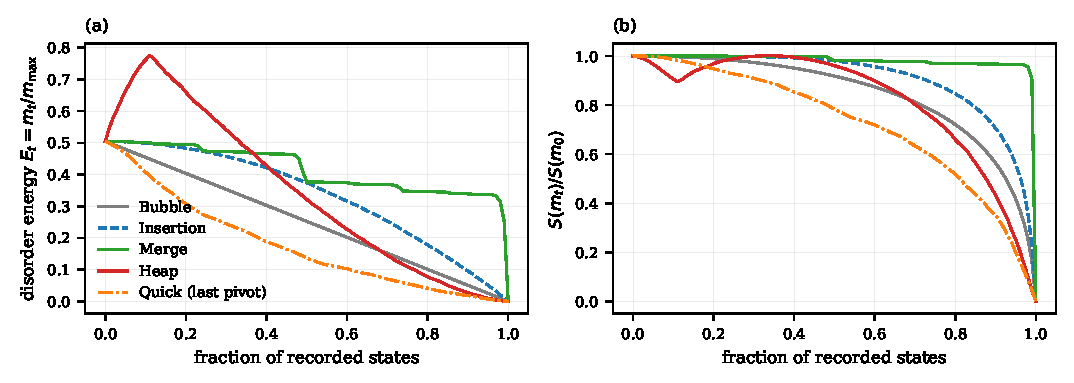
\includegraphics[width=\textwidth]{fig/trajectories.pdf}
\caption{Mean trajectories over 30 uniform-random inputs at $n=100$, against the fraction of recorded states. (a)~Disorder energy $E_t$. (b)~Exact entropy $S(m_t)$ relative to its initial value. Heap Sort is the only algorithm whose $E$ rises and whose entropy first falls.}
\label{fig:traj}
\end{figure*}

\begin{table}[!t]
\centering
\caption{Trajectory statistics at $n=100$ (30 uniform-random inputs).}
\label{tab:traj}
\scriptsize
\setlength{\tabcolsep}{3.5pt}
\begin{tabular}{@{}lrrrrr@{}}
\toprule
Algorithm & Steps & Incr.\ (\%) & Peak $E$ & Max drop (\%$m_0$) & $\Lambda$ \\
\midrule
Bubble & $2497.7$ & $0.0$ & $0.505$ & $0.04$ & $1.002$ \\
Insertion & $99.0$ & $0.0$ & $0.505$ & $3.55$ & $1.002$ \\
Merge & $99.0$ & $0.0$ & $0.505$ & $50.72$ & $1.002$ \\
Heap & $580.9$ & $83.0$ & $0.786$ & $7.36$ & $3.284$ \\
Quick (last pivot) & $282.6$ & $0.0$ & $0.505$ & $3.96$ & $1.002$ \\
\bottomrule
\end{tabular}
\end{table}

\subsection{Cost at $n=100$}
Table~\ref{tab:cost} gives $W$ and $R$ over 1000 paired trials. On uniform-random input the order by cost is Quick (1486), Merge (1886), Heap (2772), Insertion (5154), Bubble (12321). Merge Sort's cost is nearly data-independent (standard deviation $5.8$, from comparisons only, since its writes are fixed at $M(100)=1344$ by the recurrence $M(n)=M(\lceil n/2\rceil)+M(\lfloor n/2\rfloor)+2n$). On nearly-sorted input the order among the five original algorithms changes to Insertion (801), Merge (1798), Quick (2654), Heap (2978), Bubble (5050), so last-pivot Quick Sort moves from first to third; its cost is $2.3$ times that of the random-pivot and median-of-three variants (1159 and 1162), consistent with the entropy-of-pivot-source picture~\cite{ref7}. On reverse-sorted input the order is Merge (1660), Heap (2492), Quick (5100), Insertion (9999), Bubble (19800); Quick Sort's comparison count reaches its maximum $\binom{100}2=4950$ while its writes are only 150. The ranking by mean $R$ is identical to the ranking by mean $W$ in every distribution, as Proposition~\ref{prop:R} leads one to expect.

\begin{table*}[!t]
\centering
\caption{Mean $\pm$ standard deviation at $n=100$ over 1000 paired trials. $W=C+M$; $R$ in units of $10^{-4}$. Reverse-sorted is deterministic (one trial; $^\dagger$ one random-pivot draw). $R$ is undefined for few-unique input.}
\label{tab:cost}
\scriptsize
\setlength{\tabcolsep}{4pt}
\begin{tabular}{@{}lrrrrrrr@{}}
\toprule
 & \multicolumn{2}{c}{Uniform-random} & \multicolumn{2}{c}{Nearly-sorted} & \multicolumn{2}{c}{Reverse-sorted} & \multicolumn{1}{c}{Few-unique} \\
\cmidrule(lr){2-3}\cmidrule(lr){4-5}\cmidrule(lr){6-7}\cmidrule(l){8-8}
Algorithm & \multicolumn{1}{c}{$W$} & \multicolumn{1}{c}{$R$} & \multicolumn{1}{c}{$W$} & \multicolumn{1}{c}{$R$} & \multicolumn{1}{c}{$W$} & \multicolumn{1}{c}{$R$} & \multicolumn{1}{c}{$W$} \\
\midrule
Bubble & $12{,}321\pm549.4$ & $0.406\pm0.011$ & $5{,}050\pm908.8$ & $0.118\pm0.022$ & $19{,}800$ & $0.505$ & $10{,}621\pm539.7$ \\
Insertion & $5{,}154\pm349.8$ & $0.972\pm0.003$ & $801\pm191.8$ & $0.745\pm0.072$ & $9{,}999$ & $1.000$ & $4{,}154\pm332.4$ \\
Merge & $1{,}886\pm5.8$ & $2.657\pm0.189$ & $1{,}798\pm21.9$ & $0.338\pm0.105$ & $1{,}660$ & $6.024$ & $1{,}868\pm8.9$ \\
Heap & $2{,}772\pm31.2$ & $1.808\pm0.139$ & $2{,}978\pm14.8$ & $0.205\pm0.066$ & $2{,}492$ & $4.013$ & $2{,}378\pm70.0$ \\
Quick (last pivot) & $1{,}486\pm165.9$ & $3.412\pm0.438$ & $2{,}654\pm623.7$ & $0.245\pm0.104$ & $5{,}100$ & $1.961$ & $1{,}607\pm116.4$ \\
Quick (median-of-3) & $1{,}590\pm115.5$ & $3.167\pm0.309$ & $1{,}162\pm173.5$ & $0.524\pm0.154$ & $2{,}174$ & $4.600$ & $2{,}168\pm128.3$ \\
Quick (random pivot) & $1{,}645\pm164.3$ & $3.074\pm0.360$ & $1{,}159\pm115.6$ & $0.524\pm0.157$ & $1{,}710^\dagger$ & $5.848$ & $1{,}853\pm110.4$ \\
Natural merge & $1{,}768\pm27.0$ & $2.835\pm0.205$ & $1{,}119\pm85.9$ & $0.543\pm0.163$ & $1{,}791$ & $5.583$ & $1{,}715\pm23.2$ \\
\bottomrule
\end{tabular}
\end{table*}

\subsection{Scaling with $n$ and crossovers}
Table~\ref{tab:sweep} and Fig.~\ref{fig:cost} show mean cost against $n$. For this implementation the expected Insertion Sort cost on random input is exactly $\mathbb{E}[W_{\mathrm{ins}}]=n(n-1)/2+2(n-1)-(H_n-1)$, since writes equal inversions plus $n-1$ and comparisons equal inversions plus $n-1$ minus the number of prefix minima ($\mathbb{E}[\text{prefix minima}]=H_n-1$, where $H_n$ is the $n$th harmonic number); it gives $5143.8$ at $n=100$ against $5153.9\pm11.1$ (standard error) measured. In the fine sweep Insertion Sort is already more expensive than Quick Sort at $n=10$ ($61.5$ against $53.5$), becomes more expensive than Merge Sort at $n=23$ ($292.7$ against $289.3$, 400 trials; it is cheaper at $n\le 22$) and more expensive than Heap Sort between $n=35$ and $n=40$. The near-tie between Insertion and Quick Sort in a single small trial is therefore not typical. On nearly-sorted input last-pivot Quick Sort degrades relative to the pivot variants as $n$ grows ($103{,}462$ against $52{,}797$ for random pivot at $n=2000$). On few-unique input it is cheapest at $n=100$ (1607) but grows quadratically thereafter ($106{,}092$ at $n=1000$ and $412{,}327$ at $n=2000$, a factor $3.9$), because with $k=5$ values a $\le$-pivot Lomuto partition leaves all keys equal to the pivot on one side.

\begin{figure*}[!t]
\centering
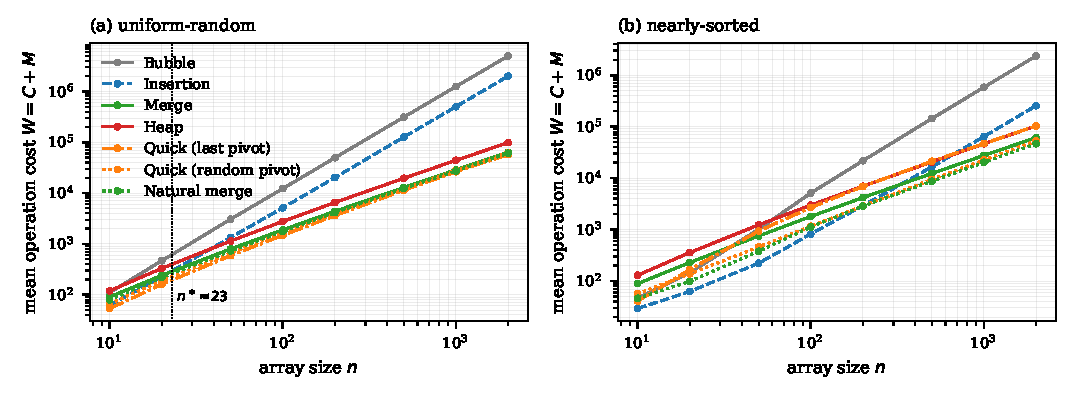
\includegraphics[width=\textwidth]{fig/cost_vs_n.pdf}
\caption{Mean cost $W=C+M$ against $n$ on log--log axes: (a)~uniform-random, with the Insertion/Merge crossover marked; (b)~nearly-sorted.}
\label{fig:cost}
\end{figure*}

\begin{table*}[!t]
\centering
\caption{Mean cost $W=C+M$ on uniform-random input for increasing $n$ (100 trials for $n\le500$, 30 for $n\ge1000$).}
\label{tab:sweep}
\scriptsize
\setlength{\tabcolsep}{6pt}
\begin{tabular}{@{}lrrrrrrrr@{}}
\toprule
Algorithm & \multicolumn{1}{c}{$n=10$} & \multicolumn{1}{c}{20} & \multicolumn{1}{c}{50} & \multicolumn{1}{c}{100} & \multicolumn{1}{c}{200} & \multicolumn{1}{c}{500} & \multicolumn{1}{c}{1000} & \multicolumn{1}{c}{2000} \\
\midrule
Bubble & $110$ & $466$ & $3{,}059$ & $12{,}264$ & $49{,}463$ & $312{,}448$ & $1{,}247{,}663$ & $4{,}989{,}747$ \\
Insertion & $62$ & $226$ & $1{,}339$ & $5{,}117$ & $20{,}201$ & $126{,}463$ & $501{,}237$ & $1{,}999{,}073$ \\
Merge & $91$ & $239$ & $794$ & $1{,}886$ & $4{,}370$ & $12{,}832$ & $28{,}669$ & $63{,}309$ \\
Heap & $119$ & $330$ & $1{,}139$ & $2{,}769$ & $6{,}538$ & $19{,}547$ & $44{,}108$ & $98{,}208$ \\
Quick (last pivot) & $53$ & $160$ & $587$ & $1{,}476$ & $3{,}598$ & $11{,}328$ & $26{,}264$ & $57{,}525$ \\
Quick (median-of-3) & $72$ & $192$ & $645$ & $1{,}574$ & $3{,}768$ & $11{,}378$ & $25{,}578$ & $57{,}478$ \\
Quick (random pivot) & $67$ & $187$ & $659$ & $1{,}633$ & $3{,}903$ & $12{,}180$ & $27{,}895$ & $62{,}230$ \\
Natural merge & $79$ & $219$ & $728$ & $1{,}768$ & $4{,}153$ & $12{,}353$ & $27{,}279$ & $60{,}578$ \\
\bottomrule
\end{tabular}
\end{table*}

\subsection{Run structure and natural merge}
The run-based entropy of ascending runs, with logarithms to base two, averages $5.51$ bits for uniform-random arrays, $2.89$ for nearly-sorted, $5.18$ for few-unique and $6.64$ for reverse-sorted (ascending runs only, so descending input is maximally fragmented). Natural merge sort reduces cost most where run entropy is low: relative to standard Merge Sort it is $6\%$ cheaper on uniform-random input, $38\%$ cheaper on nearly-sorted input ($1119$ against $1798$, $R=0.543\times10^{-4}$ against $0.338\times10^{-4}$), and $8\%$ more expensive on reverse-sorted input, where its ascending-run detection finds nothing to exploit. At $n=100$ Insertion Sort is still cheaper on nearly-sorted input ($801$), but natural merge overtakes it by $n=200$ ($2852$ against $2909$) and is cheapest at $n=500$ ($8690$ against $16{,}544$), in line with the run-based analysis of~\cite{ref5}.

\subsection{Effective inverse temperature along trajectories}
\label{sec:res-temp}
Table~\ref{tab:ensemble} checks the canonical ensemble of Section~\ref{sec:ensemble} against the exact landscape at $n=100$: as $\beta$ increases from $-20$ to $400$, the modal $m$ moves monotonically down from $2590$ to $934$, $\langle E\rangle_\beta$ tracks it, and $\beta_{\mathrm{eff}}$ evaluated at the mode recovers the input $\beta$ to within rounding, confirming~\eqref{eq:betaeff} as the corresponding local inverse-temperature relation. $\beta=0$ reproduces the uniform distribution exactly ($\langle E\rangle_0=0.500$, mode $m=2475$).

\begin{table}[!t]
\centering
\caption{Exact canonical ensemble at $n=100$: for each $\beta$, the mean and modal disorder, the corresponding $\beta_{\mathrm{eff}}$, and the free energy $F=-\beta^{-1}\ln Z(\beta)$.}
\label{tab:ensemble}
\footnotesize
\setlength{\tabcolsep}{5pt}
\begin{tabular}{@{}rrrrr@{}}
\toprule
$\beta$ & $\langle E\rangle_\beta$ & mode $m$ & $\beta_{\mathrm{eff}}$ at mode & $F(\beta)$ \\
\midrule
$-20$ & $0.523$ & $2590$ & $-20.01$ & $18.698$ \\
$-10$ & $0.511$ & $2533$ & $-10.08$ & $36.880$ \\
$0$ & $0.500$ & $2475$ & $0.00$ & --- \\
$10$ & $0.489$ & $2417$ & $10.08$ & $-35.880$ \\
$20$ & $0.477$ & $2360$ & $20.01$ & $-17.698$ \\
$50$ & $0.443$ & $2190$ & $50.03$ & $-6.803$ \\
$100$ & $0.389$ & $1922$ & $99.99$ & $-3.194$ \\
$200$ & $0.300$ & $1475$ & $200.10$ & $-1.426$ \\
$400$ & $0.190$ & $934$ & $400.19$ & $-0.594$ \\
\bottomrule
\end{tabular}
\end{table}

We then evaluate $\beta_{\mathrm{eff}}$ along the 30 uniform-random trajectories of Section~\ref{sec:res-temp2} at $n=100$. Because Bubble, Insertion, Merge and Quick Sort never increase $m$ (Section~\ref{sec:struct}), the most extreme macrostate any of them visits is $m_0$ itself, so the most negative $\beta_{\mathrm{eff}}$ on each of their trajectories occurs at $m_0$: a mean $\beta_{\mathrm{eff}}(m_0)=-3.89$ over the 30 inputs, close to zero because $E_0$ is itself close to the entropy peak. Heap Sort reaches a substantially more negative inverse-temperature regime: its most negative recorded state has a mean $\beta_{\mathrm{eff}}=-343.2$ (minimum $-414.6$ over the 30 inputs), nearly two orders of magnitude larger in magnitude than the monotone algorithms' mean, and $33.3\%$ of its recorded states lie at negative $\beta_{\mathrm{eff}}$ against $2.9$--$17.2\%$ for the other four (Table~\ref{tab:traj-temp}). This is the same asymmetry Section~\ref{sec:res-temp2} reports as $\Lambda$, now expressed on the ensemble's inverse-temperature scale rather than as a path length: Heap Sort's heap-construction phase pushes the array toward low-multiplicity, high-disorder macrostates on the far side of the entropy peak.

\begin{table}[!t]
\centering
\caption{Effective inverse temperature along trajectories at $n=100$ (30 uniform-random inputs). $\beta_{\mathrm{eff}}$ at the most negative recorded state per trial, then averaged.}
\label{tab:traj-temp}
\scriptsize
\setlength{\tabcolsep}{3.5pt}
\begin{tabular}{@{}lrrr@{}}
\toprule
Algorithm & Neg.-$\beta$ steps (\%) & Mean most-neg.\ $\beta_{\mathrm{eff}}$ & Min.\ $\beta_{\mathrm{eff}}$ \\
\midrule
Bubble & $3.1$ & $-3.89$ & $-50.56$ \\
Insertion & $12.8$ & $-3.89$ & $-50.56$ \\
Merge & $17.2$ & $-3.89$ & $-50.56$ \\
Heap & $33.3$ & $-343.23$ & $-414.61$ \\
Quick (last pivot) & $2.9$ & $-3.89$ & $-50.56$ \\
\bottomrule
\end{tabular}
\end{table}
\FloatBarrier

\section{Discussion}
\subsection{What the framework adds}
Because $E_f=S_f=0$ for every complete sort, endpoint quantities are identical across algorithms and $R=E_0/W$ carries no more ranking information than $W$ (Proposition~\ref{prop:R}). What the framework adds is the path: the exact step-by-step description of Section~\ref{sec:struct}, the excursion and drop-size statistics, the entropy path length $\Lambda$, and the effective inverse temperature $\beta_{\mathrm{eff}}$ of Section~\ref{sec:res-temp}, all functions of $S(m)$ rather than of $m$ or $E$ alone. Bubble, Insertion, Merge and Quick Sort all move monotonically downward in $m$, at costs that differ by a factor of eight, while Heap Sort's $\Lambda=3.28$ and $\beta_{\mathrm{eff}}\approx-343$ at its most negative point record a genuine excursion into a much lower-multiplicity region of permutation space. The distinction is not quantified by $m$ or $E$ alone: a peak of $E\approx0.79$ identifies the excursion in disorder but does not quantify how far it lies from the high-multiplicity centre of the entropy landscape. Comparing a positional macrostate with a structural one, such as run entropy~\cite{ref5}, is a natural way to extend this.

\subsection{Relation to physical energy}
$W$ is an abstract operation count, not energy. Studies that measure energy on devices, on smartphones~\cite{ref22}, on Android~\cite{ref23}, in Java~\cite{ref27}, in meta-analysis~\cite{ref26} and across implementation languages and input patterns~\cite{ref32}, or that treat energy-efficient sorting algorithmically~\cite{ref21,ref29}, provide the natural way to test whether $W$, with a weight on writes as in~\cite{ref19}, predicts measured energy. We do not attempt that here. On the theory side, connecting a per-run entropy path to the stochastic thermodynamics of computation~\cite{ref28,ref31} would require a physical model of the machine, and the classical bounds~\cite{ref9,ref10,ref18,ref20,ref25} remain background only.

\subsection{Limitations and threats to validity}
Each algorithm is a single implementation, and pivot rule and merge scheme matter, as the variants show. Costs are abstract counts in Python-level accounting, weighted equally; a swap is charged three writes by convention. The entropy analysis assumes distinct keys, so few-unique input is reported only through $C$, $M$ and $W$. The trajectory results use 30 inputs at $n=100$ on uniform-random input; they are fully explained by the structural propositions but not sampled across all distributions. The random-pivot result for reverse-sorted input is a single draw. Sizes stop at $n=2000$, and the nearly-sorted generator produces one particular family of low-disorder inputs.

\subsection{Future work}
Two directions follow directly. First, other representations of inversion structure, including inversion sequences with pattern restrictions~\cite{ref24} and sorting operations acting on inversion sequences~\cite{ref30}, suggest tracking the entropy of the inversion-sequence representation instead of $m$. Second, run-based macrostates that count descending as well as ascending runs~\cite{ref5} should remove the reverse-sorted penalty of the natural merge sort used here, and a sweep over the write weight $\lambda$ in $W=C+\lambda M$ would test how sensitive the rankings are to the read/write asymmetry~\cite{ref19}.

\section{Conclusion}
We described sorting runs as trajectories through an exactly computed entropy landscape on inversion-count macrostates. The step-level behaviour of each algorithm is characterised exactly. The $n=100$ cost experiments use $10^3$ paired trials, while the trajectory experiment uses 30 uniform-random inputs; in the latter, Heap Sort raises disorder in 83.0\% of its steps and traverses $3.3$ times its net entropy change. Cost rankings depend on input shape and size, with Insertion Sort overtaking Merge Sort at $n\approx23$ and last-pivot Quick Sort moving from cheapest to third on nearly-sorted and reverse-sorted input. The disorder reduction rate equals $E_0/W$, so it normalises rather than ranks; the entropy path is what the framework adds. The framework is abstract, and calibrating it against measured device energy is the main open step.

\appendices
\section{Reproducibility}
All numbers and figures are generated by the supplementary code~\cite{ref35} (Python 3.12, NumPy 2.4, SciPy 1.17). \texttt{states.py} computes exact Mahonian counts with Python integers; \texttt{algorithms.py} holds the instrumented sorts; \texttt{fastcount.py} the count-only versions; \texttt{exp\_main.py}, \texttt{exp\_traj.py}, \texttt{exp\_path.py} and \texttt{exp\_ensemble.py} run the experiments; \texttt{gen\_tables.py} and \texttt{figs.py} produce Tables~\ref{tab:cost}--\ref{tab:traj-temp} and the figures. The commands are \texttt{python exp\_main.py main}, \texttt{fine}, and \texttt{sweep}, followed by \texttt{python exp\_traj.py}, \texttt{exp\_path.py}, \texttt{exp\_ensemble.py}, \texttt{gen\_tables.py} and \texttt{figs.py}. The seed entropy is 20260927 throughout. The entire pipeline, including the exact $n=100$ Mahonian table (under 0.1\,s) and the canonical-ensemble check of Table~\ref{tab:ensemble}, runs in a few minutes on one CPU core.

\begin{thebibliography}{99}
\bibitem{ref1} D. E. Knuth, \emph{The Art of Computer Programming, Volume 3: Sorting and Searching}, 2nd ed. Addison-Wesley, 1998.
\bibitem{ref2} T. M. Cover and J. A. Thomas, \emph{Elements of Information Theory}, 2nd ed. Wiley-Interscience, 2006.
\bibitem{ref3} R. M. Gray, \emph{Entropy and Information Theory}, 2nd ed. Springer, 2011. [Online]. Available: \url{https://ee.stanford.edu/~gray/it.pdf}
\bibitem{ref4} J. Kahn and J. H. Kim, ``Entropy and sorting,'' \emph{J. Comput. Syst. Sci.}, vol. 51, no. 3, pp. 390--399, 1995.
\bibitem{ref5} O. Gila, M. T. Goodrich, and V. Sridhar, ``How to sort in a refrigerator: Simple entropy-sensitive strictly in-place sorting algorithms,'' in \emph{Proc. LATIN 2026}; arXiv:2603.05676 [cs.DS], 2026.
\bibitem{ref6} M. P. Schellekens, ``Entropy conservation for comparison-based algorithms,'' \emph{Topology Appl.}, vol. 309, Art. no. 107913, 2022.
\bibitem{ref7} B. List, M. Maucher, U. Sch\"oning, and R. Schuler, ``Randomized Quicksort and the entropy of the random source,'' in \emph{Computing and Combinatorics (COCOON 2005)}, LNCS vol. 3595. Springer, 2005, pp. 450--460.
\bibitem{ref8} MIT 6.006, \emph{Introduction to Algorithms}, ``Lecture 10: Sorting III: Linear bounds/linear-time sorting,'' MIT OpenCourseWare, 2008. [Online]. Available: \url{https://ocw.mit.edu/courses/6-006-introduction-to-algorithms-fall-2011/}
\bibitem{ref9} R. Landauer, ``Irreversibility and heat generation in the computing process,'' \emph{IBM J. Res. Develop.}, vol. 5, no. 3, pp. 183--191, 1961.
\bibitem{ref10} C. H. Bennett, ``Logical reversibility of computation,'' \emph{IBM J. Res. Develop.}, vol. 17, no. 6, pp. 525--532, 1973.
\bibitem{ref11} J. C. Baez and M. Stay, ``Algorithmic thermodynamics,'' \emph{Math. Struct. Comput. Sci.}, vol. 22, no. 5, pp. 771--787, 2012.
\bibitem{ref12} M. M\'ezard and A. Montanari, \emph{Information, Physics, and Computation}. Oxford Univ. Press, 2009.
\bibitem{ref13} P. A. MacMahon, \emph{Combinatory Analysis}, vol. 1. Cambridge Univ. Press, 1915.
\bibitem{ref14} R. P. Stanley, \emph{Enumerative Combinatorics, Vol. 1}, 2nd ed. Cambridge Univ. Press, 2012.
\bibitem{ref15} M. B\'ona, \emph{Combinatorics of Permutations}, 2nd ed. CRC Press, 2012.
\bibitem{ref16} B. H. Margolius, ``Permutations with inversions,'' \emph{J. Integer Sequences}, vol. 4, Art. 01.2.4, 2001.
\bibitem{ref17} E. Ben-Naim, ``On the mixing of diffusing particles,'' arXiv:1010.2563, 2010.
\bibitem{ref18} P. Faist, F. Dupuis, J. Oppenheim, and R. Renner, ``The minimal work cost of information processing,'' \emph{Nature Commun.}, vol. 6, Art. no. 7669, 2015, doi:10.1038/ncomms8669.
\bibitem{ref19} G. E. Blelloch, J. T. Fineman, P. B. Gibbons, Y. Gu, and J. Shun, ``Sorting with asymmetric read and write costs,'' in \emph{Proc. 27th ACM Symp. Parallelism Algorithms Architectures (SPAA)}, 2015, pp. 1--12, doi:10.1145/2755573.2755604.
\bibitem{ref20} A. S. Wright, ``The physics of forgetting: Thermodynamics of information at IBM 1959--1982,'' \emph{Perspectives Sci.}, vol. 24, no. 1, pp. 112--141, 2016, doi:10.1162/POSC\_a\_00194.
\bibitem{ref21} B. Geissmann and P. Penna, ``Sorting processes with energy-constrained comparisons,'' \emph{Phys. Rev. E}, vol. 97, no. 5, Art. no. 052108, 2018, doi:10.1103/PhysRevE.97.052108.
\bibitem{ref22} M. Verma and K. R. Chowdhary, ``Analysis of energy consumption of sorting algorithms on smartphones,'' \emph{SSRN Electron. J.}, 2018, doi:10.2139/ssrn.3168550.
\bibitem{ref23} A. Schuler and G. Anderst-Kotsis, ``Examining the energy impact of sorting algorithms on Android: An empirical study,'' in \emph{Proc. 16th EAI Int. Conf. Mobile Ubiquitous Syst. (MobiQuitous)}, 2019, pp. 404--413, doi:10.1145/3360774.3360808.
\bibitem{ref24} J. S. Kim and Z. Lin, ``Pattern-avoiding inversion sequences and open partition diagrams,'' \emph{Theor. Comput. Sci.}, vol. 841, pp. 186--197, 2020, doi:10.1016/j.tcs.2020.07.011.
\bibitem{ref25} I. Georgescu, ``60 years of Landauer's principle,'' \emph{Nature Rev. Phys.}, vol. 3, p. 770, 2021, doi:10.1038/s42254-021-00400-8.
\bibitem{ref26} G. Dlamini, F. Jolha, Z. Kholmatova, and G. Succi, ``Meta-analytical comparison of energy consumed by two sorting algorithms,'' \emph{Inf. Sci.}, vol. 582, pp. 767--777, 2022, doi:10.1016/j.ins.2021.09.061.
\bibitem{ref27} K. Carter, S. M. G. Ho, M. M. A. Larsen, M. Sundman, and M. H. Kirkeby, ``Energy and time complexity for sorting algorithms in Java,'' arXiv:2311.07298, 2023.
\bibitem{ref28} G. Manzano, G. Karde\c{s}, \'E. Rold\'an, and D. H. Wolpert, ``Thermodynamics of computations with absolute irreversibility, unidirectional transitions, and stochastic computation times,'' \emph{Phys. Rev. X}, vol. 14, Art. no. 021026, 2024, doi:10.1103/PhysRevX.14.021026.
\bibitem{ref29} V. Jayapaul, S. Jo, K. V. Palem, and S. R. Satti, ``Energy efficient sorting, selection and searching,'' \emph{Theor. Comput. Sci.}, vol. 1002, Art. no. 114592, 2024, doi:10.1016/j.tcs.2024.114592.
\bibitem{ref30} T. Mansour, H. Skogman, and R. Smith, ``Sorting inversion sequences,'' \emph{Discrete Math. Theor. Comput. Sci.}, vol. 27, no. 1, 2025, doi:10.46298/dmtcs.14010.
\bibitem{ref31} P. Chattopadhyay, A. Misra, T. Pandit, and G. Paul, ``Landauer principle and thermodynamics of computation,'' \emph{Rep. Prog. Phys.}, vol. 88, no. 8, Art. no. 086001, 2025, doi:10.1088/1361-6633/add6b3.
\bibitem{ref32} M. S. Islam \emph{et al.}, ``Cross-language evaluation of sorting algorithms on various input patterns: A comparative study,'' \emph{J. Comput. Lang.}, vol. 87, Art. no. 101397, 2026, doi:10.1016/j.cola.2026.101397.
\bibitem{ref33} H. Mannila, ``Measures of presortedness and optimal sorting algorithms,'' \emph{IEEE Trans. Comput.}, vol. C-34, no. 4, pp. 318--325, 1985.
\bibitem{ref34} V. Estivill-Castro and D. Wood, ``A survey of adaptive sorting algorithms,'' \emph{ACM Comput. Surv.}, vol. 24, no. 4, pp. 441--476, 1992.
% TODO: after the Zenodo release, replace the URL below with the DOI link (https://doi.org/10.5281/zenodo.XXXXXXX).
\bibitem{ref35} P. Mishra, ``Supplementary code and data for `Entropy landscapes and kinetics of classical sorting algorithms','' 2026. [Online]. Available: \url{https://github.com/punyajitmishra/entropy-sorting-landscapes}
\end{thebibliography}

\end{document}
